%% Latex template for PhD dissertation or MS thesis
%% Electrical and Computer Engineering Department
%% Brigham Young University
%% Last Modified:  March 2012

\documentclass[12pt]{report}

%%%%%%%%%%%%%%%%%%%%%%%%%%%%%%%%%%%%%%%%%%%%%%%%%%%%%%%%
%  Setup BYU thesis format
%%%%%%%%%%%%%%%%%%%%%%%%%%%%%%%%%%%%%%%%%%%%%%%%%%%%%%%%%
\usepackage{byustyle}
% Setup the byu style sheet
\byustylesetup{%
    %
    %isdissertation = true,            % Uncomment this if you're doing a PhD dissertation
    %etdsubmission = true,            % Uncomment this if you're compiling it for ETD submission
    singlepageabstract = true, % Comment this out if your abstract is multiple pages
    singlepageacknowledgements = true, % Uncomment this if your Acknowledgements is multiple pages
    %
    % Definitions of names needed in thesis/dissertation
    deptname          = Department of Electrical and Computer Engineering,    %
    collegename       = Ira A. Fulton College of\\Engineering and Technology, %
    committeechairman = Firstname Mi. Lastname,                      %
    committeemembera  = Firstname Mi. Lastname,                         %
    committeememberb  = Firstname Mi. Lastname,                          %
    %committeememberc  = Firstname Mi. Lastname,                    % PhD Only
    %committeememberd  = Firstname Mi. Lastname,                     % PhD Only
    graddate = April 2013,  % Leave commented for current month and year
    %copyrightyear = 2012,      % Leave commented for current year
    % uncomment the keywords for a dissertation
    %keywords         = {elecromagnetic waves, crazy circuits}
    %
    % Uncomment to shorten for proofreading purposes
    %noabstract = true,         % Don't show the abstract page
    %nouniversitypages = true,  % Don't show any of the "university pages"
    %noacknowledgements = true, % Don't show the Acknowledgements page
    %notableofcontents = true,  % Don't show the Table of Contents
    %nolistoffigures = true,    % Don't show the List of Figures
    %nolistoftables = true,     % Don't show the List of Tables
    %notocandlists = true,      % Don't show the Table of Contents, List of Figures, or the List of Tables
    %noheaderatall = true,      % Don't show any of the BYU Thesis header pages
}
%%%%%%%%%%%%%%%%%%%%%%%%%%%%%%%%%%%%%%%%%%%%%%%%%%%%%%%%
%  END:  Setup BYU thesis format
%%%%%%%%%%%%%%%%%%%%%%%%%%%%%%%%%%%%%%%%%%%%%%%%%%%%%%%%%

%%%%%%%%%%%%%%%%%%%%%%%%%%%%%%%%%%%%%%%%%%%%%%%%%%%%%%%%
%  Include other \usepackage{} statements here.
%    Add one package at a time.
%    Warning:  Some packages are not compatible with byuthesis.sty
%%%%%%%%%%%%%%%%%%%%%%%%%%%%%%%%%%%%%%%%%%%%%%%%%%%%%%%%%
%\usepackage[normalmargins]{savetrees} % prints smaller to save trees (draft only)
\usepackage{amsmath,amssymb} % math definitions
\usepackage{graphicx}        % for figures
\usepackage{subfigure}       % for figures with multiple subfigures
\usepackage{setspace}        % so all the captions will be single spaced
%%%%%%%%%%%%%%%%%%%%%%%%%%%%%%%%%%%%%%%%%%%%%%%%%%%%%%%%
%  END: Include other \usepackage{} statements here.
%%%%%%%%%%%%%%%%%%%%%%%%%%%%%%%%%%%%%%%%%%%%%%%%%%%%%%%%%

%%%%%%%%%%%%%%%%%%%%%%%%%%%%%%%%%%%%%%%%%%%%%%%%%%%%%%%%
% For doing bookmarks in the PDF file
%%%%%%%%%%%%%%%%%%%%%%%%%%%%%%%%%%%%%%%%%%%%%%%%%%%%%%%%%
% For more info, see:
% http://www.geocities.com/kijoo2000/latex2pdf.pdf
% http://www.tug.org/applications/hyperref/manual.html
\usepackage[dvipdfm,backref,pagebackref,plainpages=false]{hyperref}
\hypersetup{
    %bookmarks    = true, % Make bookmarks (default=true). This option
                          %cannot be used after package has been loaded,
                          %thus use like this: \usepackage[bookmarks=false]{hyperref}.
    %
    breaklinks   = false, % Allow link text to break across lines (default=false).
    linktocpage  = false, % make page number, not text, be link on TOC, LOF and LOT
    colorlinks   = false, % Color the text of links (true) or put color frames over
                          % the links (false).
% NOTE: if you need to use a dvi->ps->pdf path for things like PSTricks, you
% may find that commenting out the next line is necessary.
    pdfborder    = 001,   % sets the default for pdf links
    pdfstartview = {FitH}, % Set the startup page view. Possible options are:
                           % FitH: Fit whole width of page
                           % FitV: Fit whole height of page
                           % FitB: Fit whole �Bounding Box� page
                           % FitBH: Fit whole width of �Bounding Box� of page
                           % FitBV: Fit whole height of �Bounding Box� of page
    bookmarksnumbered  = true, % Put section numbers in bookmarks (default=false)
    bookmarksopen      = true, % Open up the bookmark trees (default=false).
    bookmarksopenlevel = 1, % Level to which bookmarks are open (default=\maxdimen).
    bookmarkstype      = toc, % Specify which toc file to mimic (default=toc).
    pdfpagemode        = {UseOutlines}, %  Specify how document starts when opened ({None}).
                                        % Possible options are:,
                                        % None: Neither bookmarks nor thumbnails are visible.
                                        % UseOutlines: Bookmarks are visible.
                                        % UseThumbs: Thumbnails are visible.
                                        % FullScreen: Full-screen mode
    pdftitle    = {Thesis Template},
    pdfauthor   = {Firstname Lastname},
    pdfcreator  = {Firstname Lastname},
    pdfsubject  = {Firstname Lastname's Master's Thesis},
    pdfkeywords = {Thesis Template, BYU},
}
%%%%%%%%%%%%%%%%%%%%%%%%%%%%%%%%%%%%%%%%%%%%%%%%%%%%%%%%
%  END: For doing bookmarks in the PDF file
%%%%%%%%%%%%%%%%%%%%%%%%%%%%%%%%%%%%%%%%%%%%%%%%%%%%%%%%%

%%%%%%%%%%%%%%%%%%%%%%%%%%%%%%%%%%%%%%%%%%%%%%%%%%%%%%%%
%                Macros
%  Define macros here
%%%%%%%%%%%%%%%%%%%%%%%%%%%%%%%%%%%%%%%%%%%%%%%%%%%%%%%%%
\def\proof{\noindent{\it Proof: }}
\def\QED{\mbox{\rule[0pt]{1.5ex}{1.5ex}}}
\def\endproof{\hspace*{\fill}~\QED\par\endtrivlist\unskip}
%
\newcommand{\norm}[1]{\left\|#1\right\|}
\newcommand{\abs}[1]{\left|#1\right|}
\newcommand{\defeq}{\stackrel{\triangle}{=}}
\newcommand{\re}{\mathbb{R}} % real numbers
\newcommand{\OMIT}[1]{{}} % omit sections of text
\newcommand{\pd}[2]{\ensuremath{\frac{\partial #1}{\partial #2}}} % partial derivative

%%%%%%%%%%%%%%%%%%%%%%%%%%%%%%%%%%%%%%%%%%%%%%%%%%%%%%%%%
%                End Macros
%%%%%%%%%%%%%%%%%%%%%%%%%%%%%%%%%%%%%%%%%%%%%%%%%%%%%%%%%

% To only print a few chapters without changing the reference numbers,
% uncomment the chapters you want
%\includeonly{intro}
%\includeonly{chapter2}
%\includeonly{appendixa}

%%%%%%%%%%%%%%%%%%%%%%%%%%%%%%%%%%%%%%%%%%%%%%%%%%%%%%%%%
% Start Document
%%%%%%%%%%%%%%%%%%%%%%%%%%%%%%%%%%%%%%%%%%%%%%%%%%%%%%%%%

\begin{document}

% Define Title & Author
\title{Brigham Young University Thesis Template}
\author{Firstname Lastname}

% For displaying the BYU Thesis header
% This command assumes that there are documents called abstract.tex and
% acknowledgements.tex that will be included in the header
\showBYUHeader


% Include chapters of the thesis here:
% each chapter should be in a file with a .tex extension and the text
% of the file should begin with \chapter{Chapter Title}, followed
% by the text of the chapter.
%  Note: the introduction is considered Chapter 1.
\chapter{Introduction}
This is an example of the introduction. It's pretty simple and shows off
some of the basic commands.

\section{First Section}
This part shows how you can divide things into sections.

\subsection{First Subsection}
Also into subsections.

\subsubsection{First Subsubsection}
And even Subsubsections but they don't work correctly with Chapters and so I
would recommend against using them.

\subsection{Second Subsection}
Which really helps organization and automatically gets added to the Table
of Contents and gets linked to by the hyperref package.

\section{Citation Example}
One of the coolest part about \LaTeX\ is BibTeX. You can just call
the $\backslash$cite command and it will do all of the bibliography
stuff for you as long as there is an entry in the refs.bib file.
Here's an example of citing previous works
\cite{SomeSweetBook06,SomeSweetArticle06}.

\section{Math and Equation Example}
Here's how to use inline math mode to define lambda like this,
$\lambda$, and how to declare Equations~\eqref{eqn:definition_Ix}
and~\eqref{eqn:definition_Iy}

\begin{equation} \label{eqn:definition_Ix}
I_x(x,y) = \pd{I(x,y)}{x},
\end{equation}

\begin{equation}\label{eqn:definition_Iy}
I_y(x,y) = \pd{I(x,y)}{y}.
\end{equation}

If you don't want equation numbers, use
\[
\text{sign}(x) = \begin{cases}
                 1,  &\quad x> 0 \\
                 -1, &\quad x<0 \\
                 0,  &\quad \text{otherwise}
                 \end{cases}.
\]


 Or you can create equation arrays like
\begin{align}
  \alpha &= \beta^\gamma \notag \\
  x &= \frac{1}{\alpha} \label{eq:cool_1} \\
  y &= \sqrt{\abs{\frac{\gamma}{\beta}}} \notag \\
  \zeta &= x^y \label{eq:cool_2}.
\end{align}


The lines in the array can be referenced by saying things like: In
Eq.~\eqref{eq:cool_1} we show a cool equation, but its not nearly as
cool as Eq.~\eqref{eq:cool_2}.

\section{Fixed Width Figure Example} \label{sec:intro_figure_example}
This part also shows how to include a basic figure like the one
shown in Figure~\ref{fig:intro_stuff}

\begin{figure}[hhhhhtb]
  \centering
  
\includegraphics[width=5.5in]{figures/intro/stuff}
  \caption[Example Fixed Width Figure]{
This figure is just a simple figure with a width set at 5.5in. An example of a
figure whose size depends on the width of the page is given in
Figure \ref{fig:appendix_some_pic} in Section \ref{sec:appendxia_figure_example}}
%
  \label{fig:intro_stuff}
\end{figure}

\section{All Done}
You know have seen a lot of the basics and now you can see some
other fancy stuff in Chapter~\ref{chp:chapter2}.

\chapter{Sample Chapter 2} \label{chp:chapter2}
This chapter shows how to use subfigure and make a table.

\section{Using the Subfigure package}
Here's an example of referencing Figure~\ref{fig:overview2} or one
of referencing Subfigure~\ref{subfig:overview2_c}
and~\ref{subfig:overview2_d}.

\begin{figure}[hhhhhtb]
  \centering
  \subfigure[First Plot]
  {
    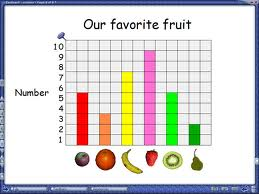
\includegraphics[width=0.4\textwidth, bb = 0 0 150 150]{figures/chapter2/a.jpg}
    \label{subfig:overview2_a}
  } \quad
  \subfigure[Second Plot]
  {
    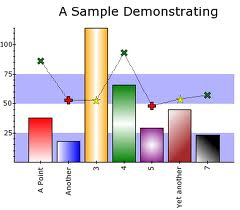
\includegraphics[width=0.4\textwidth, bb = 0 0 150 150]{figures/chapter2/b.png}
    \label{subfig:overview2_b}
  } \\
  \subfigure[Third Plot]
  {
    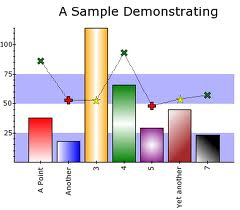
\includegraphics[width=0.4\textwidth, bb = 0 0 150 150]{figures/chapter2/c.png}
    \label{subfig:overview2_c}
  } \quad
  \subfigure[Fourth Plot]
  {
    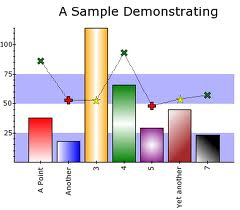
\includegraphics[width=0.4\textwidth, bb = 0 0 150 150]{figures/chapter2/d.png}
    \label{subfig:overview2_d}
  } \\
  \caption[Cool Figure from Chapter 2 made with the subfigure package]{
  This figure shows how to use PNGs and JPGs as a figure.
  %
  \subref{subfig:overview2_a} This is a groovy plot.
  %
  \subref{subfig:overview2_b} This ones cool too.
  %
  \subref{subfig:overview2_c} I don't like this one.
  %
  \subref{subfig:overview2_d} But this one is ok.}
  \label{fig:overview2}
\end{figure}


\section{Making a table}
Making a table in \LaTeX\ is a little like make one in HTML, but
with some little quirks. An example is Table~\ref{tab:comparison}.

You make a table is by starting a table environment with a caption
and label (You can specify the text that shows up in the Table of
Contents using the optional parameter box, [], that's at the
beginning of the $\backslash$caption command. You tell the table how
many columns in the beginning of the tabular environment using a
command like this |l|c|r|. That would create a table with 3 columns
that are left-aligned, centered and right-aligned, in that order. So
you can do just about anything you want. The |'s tell \LaTeX\ that
you want bars separating the columns. You can also add horizontal
lines using the $\backslash$hline command. Oh ya, and I told it to
center using the $\backslash$centering command.


\begin{table}[hhhhtbp]
\centering
\caption[Example Table]{Description of the table}
\label{tab:comparison}
%
\begin{tabular}{|l|c|c|r|}
\hline

Table Name  & Column 2 & Column 3   & Column 4 \\
\hline
First Row   & 4780286  & 72.941376  & A \\
Second Row  & 4069335  & 62.093124  & B \\
Third Row   & 4074900  & 62.178040  & C \\
\hline
Fourth Row  & 4000000  & 60.000000  & Z \\
\hline

\end{tabular}
\end{table}





%%%%%%%%%%%%% begin Bibliography %%%%%%%%%%%%%%%%%
\phantomsection %Forces a new section prior to setting the bibliography reference point
\bibliographystyle{IEEEtran}
\addcontentsline{toc}{chapter}{Bibliography}
\bibliography{refs}

% Bibliographies are best created and maintained using BibTeX
% To use Bibtex, create a bibliography file, e.g., refs.bib
% The sample file sources.bib shows examples of different
% bibliographic entries.
% The bibliography is created by executing:
%  1.  latex, 2. bibtex, 3. latex, 4. latex
%%%%%%%%%%%%%%%% end Bibliography %%%%%%%%%%%%%%%%%

%Included because WinEdit is RETARDED and it needs it for Gather Purposes:
%input "refs.bib"


% Include appendix sections here:
% each appendix should be a file with a .tex extension and the text
% of the file should begin with \appendix{Appendix Title}, followed
% by the contents of the appendix
\appendix{Sample Appendix}

\section{Width Based on Page Size Figure Example} \label{sec:appendxia_figure_example}
Here's an example of a figure whose width depends on the width
of the page. You can see if as Figure \ref{fig:appendix_some_pic}.

\begin{figure}[htbp]
  \centering
  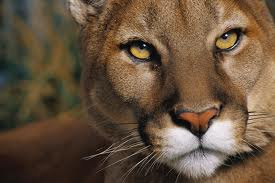
\includegraphics[width=0.45\textwidth]{figures/appendixa/some_pic}
  \caption[Example Width Based on Page Size Figure]{
    This is an example of a figure whose width will be 45\% of the
    width of the page. If you'd like to see a figure with a fixed
    width then you can see it as Figure \ref{fig:intro_stuff} in
    Section \ref{sec:intro_figure_example}. Just FYI, I made this
    figure with PowerPoint and then copied it and pasted it into
    wmf2eps and choose the "Paste EMF" option. It will generate
    a larger file, but it will look a TON better than the
    "Paste WMF" option and the "Paste DIB" option will paste the
    rasterized image that won't scale well at all.}
  \label{fig:appendix_some_pic}
\end{figure}

%End the document
\end{document}
